\documentclass[convert = false, tikz]{standalone}
\usepackage[utf8]{inputenc}
\usepackage{tikz}
\usetikzlibrary{automata, positioning, arrows}
 
\usepackage{../../../../style_automata}

\tikzset{
node distance=1.5cm, % specifies the minimum distance between two nodes.
}

\begin{document}
    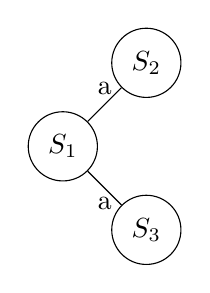
\begin{tikzpicture}
        \node[state] (s1) {$S_1$};
        \node[state, above right of=s1] (s2) {$S_2$};
        \node[state, below right of=s1] (s3) {$S_3$};
        \draw (s1) edge[above] node{a} (s2)
        (s1) edge[below] node{a} (s3);
    \end{tikzpicture}
\end{document}